% -*- TeX:UTF-8 -*-
%%
%% POSTECH 학위논문양식 LaTeX용 (ver 0.1) 예시
%%
%% @version 0.2
%% @author  박준신 Junshin Park (mailto:lonelywing@postech.ac.kr)
%% @date    2015. 8. 31.
%%
%% @requirement
%% teTeX, fpTeX, teTeX 등의 LaTeX2e 배포판
%% + 은광희 님의 HLaTeX 0.991 이상 버젼 또는 홍석호 님의 HPACK 1.0
%% : 설치에 대한 자세한 정보는 http://www.ktug.or.kr을 참조바랍니다.
%%
%% @note
%% 기존의 Kaist dissertation template을 바탕으로 작성되었습니다.
%% 현재 수정중에 있고, 버그리포트는 위 저자의 이메일로 보내주시면 감사하겠습니다.
%%
%% @acknowledgement
%% 본 latex template은 kaist 채승병님의 template을 바탕으로 만들어졌음을 밝힙니다.
%% Alpha test 및 본 thesis 예시 내용은 컴퓨터공학과 졸업생이신 오수영 학우의 도움으로 작성되었습니다.
%% -------------------------------------------------------------------
%% @information
%% 이 예제 파일은 hangul-ucs를 사용합니다. UTF-8 입력 인코딩으로
%% 작성되었습니다. hlatex의 hfont는 이용하지 않습니다. --2006/02/11

% @class kaist.cls
% @options [default: doctor, korean, final]
% - doctor: 박사과정 | master : 석사과정
% - korean: 한글논문 | english: 영문논문
% - final : 최종판   | draft  : 시험판
% - pdfdoc : 선택하지 않으면 북마크와 colorlink를 만들지 않습니다.
\documentclass[master,english,final]{postech-ucs}
% If you want make pdf document (include bookmark, colorlink)
%\documentclass[doctor,english,final,pdfdoc]{kaist-ucs}

% postech-ucs.cls 에서는 기본으로 dhucs, ifpdf, graphicx 패키지가 로드됩니다.
% 추가로 필요한 패키지가 있다면 주석을 풀고 적어넣으십시오,
%\usepackage{...}
\usepackage{amsmath}
\usepackage{enumitem}
\usepackage{algorithm}
\usepackage{algpseudocode}
\usepackage{comment}
% \usepackage{bbm}
% \renewcommand{\thealgorithm}{}
\newcommand{\argmax}{\operatornamewithlimits{arg\,max}}

% @command title 논문 제목(title of thesis)
% @options [default: (none)]
% - korean: 한글제목(korean title) | english: 영문제목(english title)
\title[korean] {파트 기반 영역 매칭을 이용한 사람 자세 추정}
\title[english]{Human Pose Estimation using Part-based Region Matching}

% @note 표지에 출력되는 제목을 강제로 줄바꿈하려면 \linebreak 을 삽입.
%       \\ 나 \newline 등을 사용하면 안됩니다. (아래는 예시)
%
%
% If you want to begin a new line in cover, use \linebreak .
% See examples above.
%


% @command author 저자 이름
% @param   family_name, given_name 성, 이름을 구분해서 입력
% @options [default: (none)]
% - korean: 한글이름 | chinese: 한문이름 | english: 영문이름
%
% If you are a foreigner (this means you have no korean name),
% Write as follow
% \author[korean]{}{}
% \author[chinese]{family name in your native language}{given name in your native language}
% \author[english]{family name in english}{given name in english}
%
\author[korean] {오}{수 영}
\author[english]{Oh}{Sueyoung}

% @command advisor 지도교수 이름 (복수가능)
% @usage   \advisor[options]{...한글이름...}{...영문이름...}{signed|nosign}
% @options [default: major]
% - major: 주 지도교수  | coopr: 공동 지도교수
\advisor[major]{한 준 희}{Joon Hee Han}{nosign}
%\advisor[coopr]{홍 길 길}{Gilgil Hong}{nosign}
%
% 지도교수 한글이름은 입력하지 않아도 됩니다.
% You may not input advisor's korean name
% like this \advisor[major]{}{Chang, Kee Joo}{signed}
%

% 현재 학과명은 카이스트템플릿으로부터 수정되지 않은 상태입니다. 추후 업데이트를 하도록 하겠습니다.
% @command department {학과이름}{학위종류} - 아래 표에 따라 코드를 입력
% @command department {department code}{degree field}
%
% department code table
%
% MA	// 수학 	Department of Mathematics
% PH	// 물리학 Department of Physics 
% CH 	// 화학 	Department of Chemistry
% LS  	// 생명과학 Department of Life Sciences
% MS 	// 신소재공학 Department of Materials Science and Engineering
% ME 	// 기계공학 Department of Mechanical Engineering
% EE 	// 전자전기공학 Department of Electrical Engineering
% IME 	// 산업경영공학 Department of Industrial & Management Engineering
% CSE 	// 컴퓨터공학 Department of Computer Science and Engineering
% CE 	// 화학공학	Department of Chemical Engineering
% CITE 	// 창의IT	Department of Creative IT Excellence Engineering
% AMS	// 첨단재료과학 Division of Advanced Material Science
% IBB 	// 시스템생명공학 Division of Integrative Bioscience and Biotechnology 
% ITCE 	// 정보전자융합 Division of IT Convergence Engineering
% ANE 	// 첨단원자력공학 Division of Advanced Nuclear Engineering
% EV 	// 환경공학	School of Environmental Science and Engineering
% IBT	// 융합생명공학과 School of Interdisciplinary Bioscience and Bioengineering
% TIM 	// 기술경영공학	Graduate Program for Technology & Innovation Management
% WE 	// 풍력특성화 School of Wind Energy
% GEM 	// 엔지니어링특성화 Graduate School of Engineering Mastership
% GIFT 	// 철강대학원 Graduate Institute of Ferrous Technology
% OSTI 	// 해양대학원 POSTECH Ocean Science & Technology Institute

%
% science: 이학 | engineering: 공학 | business : 경영학
% 박사논문의 경우는 학위종류를 입력하지 않아도 됩니다.
% If you write Ph.D. dissertation, you cannot input degree field.

\department{CSE}{engineering}

% @command studentid 학번(ID)
\studentid{20130732}

% @command referee 심사위원 (석사과정 3인, 박사과정 5인)
\referee[1]{Joon Hee Han}
\referee[2]{Daijin Kim}
\referee[3]{Ki-Sang Hong}
% \referee[5] {Barack Obama}
% Of course english name is available

% @command approvaldate 지도교수논문승인일
% @param   year,month,day 연,월,일 순으로 입력
\approvaldate{2015}{12}{24}

% @command refereedate 심사위원논문심사일
% @param   year,month,day 연,월,일 순으로 입력
\refereedate{2015}{12}{24}

% @command gradyear 졸업년도
\gradyear{2016}

% 본문 시작
\begin{document}

    % 앞표지, 속표지, 학위논문 제출승인서, 학위논문 심사완료 검인서는
    % 클래스 옵션을 final로 지정해주면 자동으로 생성되며,
    % 반대로 옵션을 draft로 지정해주면 생성되지 않습니다.

    % 영문초록 (abstract)
    \begin{abstract}
        In this thesis, a part-based region matching algorithm is proposed for human pose estimation in 2D images. A new notion of part, named a semantic part is introduced. A semantic part is represented as a combination of classic rigid parts and contains partial semantic information of body pose. Region proposals are used to form a set of candidate bounding boxes for semantic parts. These regions are matched between target and source images and their confidences are evaluated by computing the matching score. The regions with high confidence is the final semantic parts which form a body pose. Based on a data-driven approach, the final pose is estimated by getting information of joint positions from the source correspondences of the final semantic parts. Using semantic information catches more meaningful pose information and the part-based region matching has simple algorithm and performs effectively for a large number of data.
    \end{abstract}

    % 목차 (Table of Contents) 생성
    \tableofcontents

    % 표목차 (List of Tables) 생성
%    \listoftables

    % 그림목차 (List of Figures) 생성
%    \listoffigures

    % 위의 세 종류의 목차는 한꺼번에 다음 명령으로 생성할 수도 있습니다.
    %\makecontents

%% 이하의 본문은 LaTeX 표준 클래스 report 양식에 준하여 작성하시면 됩니다.
%% 하지만 part는 사용하지 못하도록 제거하였으므로, chapter가 문서 내의
%% 최상위 분류 단위가 됩니다.
%% You cannot use 'part'

\chapter{Introduction}

% Definition of Human pose estimation (or not..)

% [Nature]
% 1. Human pose estimation is still challenging problem in computer vision area.
% 2. It is applied to ~~ image understanding , ...
% 3. It is difficult problem....because human body is highly articulated.
% [Overview]
% 1. Human pose is represented as configuration of multiple body parts.
% 2. But, because human body is 1) highly articulated and because of 2) degree of freedom
% more difficult than other general object detection.
% [Related work]
% 1. General : Human pose is represented as hierarchical graph model(pictorial structure)
% appearance model / geometrical model (dependency)
% 2. FMP
% 3. ??
% [Transition]
% 1. But they fail to find highly complex pose or in case of some of parts are occluded by other part.
% 2. need to consider semantic information
% [Our work]
% 1. We proposed ~ 1) semantic part 2) patch based region matching
% 2. Idea : 1) (show example) To find crossed-arm is easier than to detect each part which consist of crossed-arm...
% 3. It is strong to self occlusion, do not need to train part detectors. avoid double-counting


Human pose estimation from a single static image is a challenging problem in computer vision. Various models for pose estimation have been proposed over the last decade and estimated human pose is applied to diverse high level vision tasks such as image understanding~\cite{imageUnderstanding:2013} and action recognition~\cite{actionRecognition:2013}.

Human pose is represented as configuration of multiple body parts, which generally are parameterized by pixel location and orientation. The estimation of human pose can be considered as a part-based object detection problem, specifically for the case of articulated objects. This means an object is modeled by a~collection of parts arranged in a deformable configuration. In terms of a problem of localization of body parts, pose estimation is more difficult problem than other general object detection because human body is highly articulated and has a large number of degrees of freedom to be estimated. The large pose variations, cluttered background, self-occlusions are challenging aspects of human pose estimation.



\chapter{Related Work}

\section{Human Pose Estimation}

\textbf{Pictorial structure }
% Genaral pose estimation (FMP,..and others)
Part-based representation is a classic framework for human pose estimation. A part-based model represents the human body as a~constellation of a set of rigid parts constrained in some fashion. Most work~\cite{pose_multiTree:2008, PS_revisited:2009, pose_latentTree:2013} on human pose estimation are graphical model-based for these body parts. In terms of part-based object detection, pose estimation is mainly represented by the pictorial structure models which is related to mixtures of parts~\cite{PS_original:2005, detection_DPM:2010}. The pictorial structure model~\cite{PS_original:2005} is efficient to solve object recognition and model learning problems. The pictorial structure decomposes the appearance of objects into local part templates, together with geometric constraints between pairs of parts. This models the spatial relations of rigid parts using usually a tree model which allows for efficient inference.


\chapter{Proposed Method}


\section{Overview}

% Introduction
The task of human pose estimation is examined in static images. Human pose estimation from a single static image is a challenging problem in computer vision. Various models for pose estimation have been proposed and a working technology is applied to diverse high level vision tasks such as image understanding~\cite{imageUnderstanding:2013} and action recognition~\cite{actionRecognition:2013}.

% Overview of general pose estimation
In general, human body pose is represented by configuration of multiple rigid parts located at joints. Body parts usually are parameterized by pixel location and orientation. The appearance of a body is decomposed into local parts, and the deformable configuration is defined with geometric constraints between a pair of parts. The goal of human pose estimation is to find every pixel location of body joints. That means to find the best configuration of multiple body parts.

The rigid parts are based on human anatomy. A human pose is labeled joint positions and they provide part positions as limbs. A body limb is represented by the joint points as endpoints of its region. In this sense, the word ``rigid parts'' appears to be used interchangeably with the expression ``joints'' and ``limbs'' here. Figure~\ref{fig:graphStructure} shows the human body model based on rigid parts.

Let $p_i \in \{p_1, \dots, p_K\}$ denote the $i$-th joint point, where $K$ is the total number of joint points. Note that we are using the expression ``rigid parts'' distinctively from the notion ``semantic part'', introduced next.


\newpage

\begin{figure}
\begin{center}
   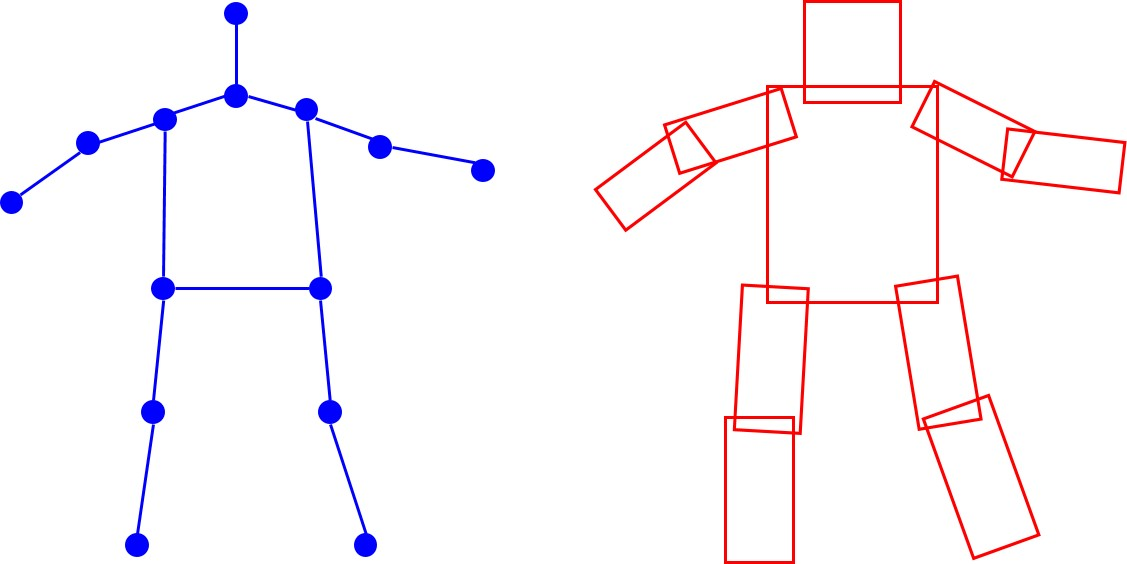
\includegraphics[width=0.8\linewidth]{./fig/graphStructure.jpg}
\end{center}
   \caption{The graph model of the articulated human body. \textbf{left}~:~Generally, human body is modeled with joint points based on human anatomy. It is parameterized by $K$~body points located at joints ($K = 14$). \textbf{right}~:~Rigid parts are represented as limbs by using the joints as endpoints of the limbs. Most previous approaches build detectors for these rigid parts. In this thesis, the final estimation is based on this human body model as the configuration of joint points, but a new approach is proposed using mid-level representation named a `semantic part', which is different from a rigid part.}
\label{fig:graphStructure}
\end{figure}

\clearpage




\section{Semantic Part}
\label{sec:semanticPart}

In most previous part-based models~\cite{FMP:2011}, rigid body parts such as head, torso, half limbs are guided by human anatomy. This representation of parts are difficult to detect accurately because single rigid part which is represented by parallel lines is not discriminative in appearance and does not contain any contextual information. This may commonly occur in clutter and induce self-occlusion. To handle large variance in appearance of human pose, the use of larger parts with more context needs to be considered. Some researches~\cite{poselet_humanParsing:2011, APM:2011, poselet_pose:2013} used larger or combined parts such as poselet~\cite{poselet_original:2009}.


\subsection{Definition}
\label{sec:semanticPart_definition}
% ---------- Definition ----------
Our notion of ``parts'' can range from basic rigid parts (e.g. torso, head, half-limb), to large pieces of bodies covering more than one rigid part. In the extreme case, the ``parts'' corresponding to the whole body. This ``part'' is named as a \emph{semantic part}. In other words, a semantic part spans multiple rigid parts (or joint points) on the body. For example, a semantic part is `head + torso', `torso + left arm' and `left leg + right leg'.

A semantic part is described as a set of one or more body limbs, in other words, subset of whole body parts. Let $S_i$ be the $i$-th semantic part, where $i$ is written as ${i \in \{1, ..., N\}}$ and $N$ is the number of semantic parts which form a~human body. We define a semantic part as:

\textbf{Definition}
\begin{eqnarray}\label{eq:semanticPart_definition_1}
S_i \in \mathcal{P} ( {p_1, \dots, p_K} ) \backslash \{\emptyset\} , && \text{for } i = 1, \dots, N
\end{eqnarray}
where $\mathcal{P} \left( \cdot \right)$ denotes the power set, the set of all subsets of a set. A semantic part is one of elements of the power set of all joint points $\{p_1, \dots, p_K\}$, excluding the empty set. This involves that in the extreme case, a semantic part can even be a~rigid part or the whole body.

However, Definition~\ref{eq:semanticPart_definition_1} occurs disconnected composition of joints. The disconnected composition cannot be considered semantically meaningful and this cannot even be represented within a image patch. Accordingly, more strict definition for a semantic part is necessary. The new definition of a semantic part is written as follows.

\textbf{Definition}
\begin{eqnarray}\label{eq:semanticPart_definition_2}
S_i \in \{G' | G' \text{ is a connected component of graph } G\} , & \text{for } i = 1, \dots, N
\end{eqnarray}



\subsection{Criteria of Semantic Part}
The term semantic part is used to describes a part of a human pose. According to our intention, we argue that a ``good'' semantic part must satisfy the criteria as in the following.

\begin{enumerate}[noitemsep]
    \item It should be easy to find semantic part given the input image. This suggests that the semantic part must be discriminative in appearance.
    \item A semantic part should be contain sufficiently semantic information. This means that the semantic part muse be semantically discriminative with the appearance.
\end{enumerate}

The criteria above involves the relation between semantics and appearance of the semantic part. In brief, the semantic part must be discriminative in both semantics and appearance. Semantic information of human pose in an image is interpreted as the geometry relation of joint positions. In next section, how the semantic parts are selected with consideration of the relation between appearance and geometry information in human poses is described.


\newpage

\subsection{Semantic Part Selection Algorithm }
\label{sec:semanticPart_algorithm}
% Introduction

\begin{algorithm}
\caption{Semantic part selection}
\label{algo:semanticPart}
\begin{algorithmic}[1]
\State Set candidates of semantic parts as combinations of rigid parts.
\State Sample patches of semantic parts, from each image of dataset.
\State Extract appearance/geometry features from the patches.
\State Compute similarities between every pair of the patches, for each appearance/geometry feature.
\State Compute correlation between appearance and geometry features, for each semantic part.
\State Select semantic parts which have high correlation.
\end{algorithmic}
\end{algorithm}


\begin{table}
\begin{center}
\begin{tabular} {lcccc}
\hline
Semantic part & left legs/arms & right legs/arms & \textbf{head+torso+arms} & \textbf{legs} \\
\hline
Correlation  &  0.408 &  0.399 & 0.391 & 0.383 \\
\hline
\end{tabular}
\end{center}
\caption{Semantic parts with high correlation. Bold~:~the semantic parts used in our experiments. \newline}
\label{tab:result_semPrt_correlation_1}

\begin{center}
\begin{tabular} {lcccc}
\hline
Semantic part & right arms & arms & left lower arm & right lower arm \\
\hline
Correlation  &  0.163 &  0.119 & 0.071 & 0.067 \\
\hline
\end{tabular}
\end{center}
\caption{Semantic parts with low correlation}
\label{tab:result_semPrt_correlation_2}

\end{table}


\chapter{Experiment}
% from IDPR
% This section introduces the datasets, clarifies the evaluation metrics, describes our experimental setup, presents comparative evaluation results.

\section{Datasets}

Experiments are performed on two standard pose estimation benchmarks: the Leed Sports Pose (LSP) dataset~\cite{dataset_LSP:2010} and the Image Parse dataset~\cite{dataset_Parse:2007}.
The LSP dataset contains 2000 pose annotated images, that contains 1000~training and 1000~test images from sport activities with annotated full-body human poses. The Parse dataset contains 305~pose-annotated images of highly articulated full body images of human poses. The Parse dataset is not a good dataset for the proposed data-driven approach, because the number of the images is too small. Experiments in this thesis are performed mostly on LSP dataset which contains relatively enough number of image data among human pose datasets. As the images have low resolution and contain partially occluded people with all kinds of poses and viewpoints, our test is challenging. Both datasets included a standard train/test split. For the proposed model, the training set are used for source images and the test set for target images.


\begin{comment}
\textbf{PCK} We used two measures for pose estimation that
\textbf{APK} In a real system, one will not have access to annotated bounding boxes at test time, and so must address the detection problem as well. On can cleanly combine the two problems by thinking of body parts (or rather joints) as objects to detected, and evaluate object detection accuracy with a precision-recall curve. We deem a candidate to be correct (true positive) if it lies within
\end{comment}

\begin{comment}
\textbf{Joint localization error }
We measure the joint localization error introduced in \cite{pose_jointRegressor:2013} as a fraction of the body size. The joint localization error is well used in other computer vision tasks such as fiducial point detection. It is independent of the actual size of the image and more precise than PCP measures which derived from bounding box-based object detection.
\end{comment}


\chapter{Result}
\label{sec:result}
\section{Quantitative Result}

% ------------ Comparison with prior works
Proposed method is compared to the state-of-the-art method~\cite{FMP:2011} that uses a flexible mixture of parts modeled by linear SVMs. The available source code published by~\cite{FMP:2011} are used. To compare with other previous work using part detectors, a joint representation is converted into a limb representation by using the joints as endpoints of the limbs. 


\chapter{Conclusion}

A part-based region matching method is proposed to estimate human poses in 2D images. As the elements of matching, a semantic part, a new part representation which is a combination of classic rigid parts is introduced. A semantic part is expected to contain sufficient semantic information of human pose. They are easier to be detected rather than detecting rigid parts which is represented by parallel lines and not discriminative in appearance.
A part-based matching between source and target regions is performed for human pose estimation. A set of candidate bounding boxes are generated from the target image by extracting object proposals, which restrict the search space. The matching algorithm evaluates matches between two sets of regions by considering both appearance and spatial consistency. The matching algorithm leads to maximize the total score for the final pose. The total score is computed by region confidences on each joint point. Finally, several best matches of regions are selected as semantic parts to form final human pose. By inferring the pose information from the source regions of the best match, every joint positions for whole body pose can be estimated.



%%
%% 한글요약문 시작 (Korean summary)
%%
%% Note. 영문논문일 경우에만 필요하니 한글논문의 경우에는 작성하지 마십시오.
%%
\begin{summarykorean}
본 논문은 2차원 영상에서 사람 자세 추정(human pose estimation)을 위해 1)~신체 파트를 관절 단위가 아닌 의미적 영역으로 구분하고, 2)~파트 검출기를 학습하는 대신 파트 기반의 영역 매칭 알고리즘(part-based region matching)을 제안한다.

	
\end{summarykorean}

%%
%% 참고문헌 시작
%% Refences
%%

\bibliographystyle{unsrt}
\bibliography{mybib}

%%
%% 감사의 글 시작
%% Acknowledgement
%%
% @command acknowledgement 감사의글
% @options [default: 클래스 옵션 korean|english ]
% - korean : 한글타이틀 | english : 영문타이틀

\acknowledgement[korean]

    때로는 엄하고 때로는 부드러운 모습으로 지도 해주신 한준희 교수님, 감사드립니다.
%%
%% 이력서 시작
%% Curriculum Vitae
%%
% @command curriculumvitae 이력서
% @options [default: 클래스 옵션 korean|english ]
% - korean : 한글이력서 | english : 영문이력서
\curriculumvitae[korean]

    % @environment personaldata 개인정보
    % @command     name         이름
        % input data only you want
    \begin{personaldata}
        \name       {Sueyoung Oh}
    \end{personaldata}

    % @environment education 학력
    % @options [default: (none)] - 수학기간을 입력
    \begin{education}
        \item[2009. 3.\ --\ 2013. 2.] Department of Computer Science and Engineering, Inha University (B.S.)
        \item[2013. 3.\ --\ 2016. 2.] Department of Computer Science and Engineering, Pohang University of Science and Technology (M.S.)
    \end{education}

    % @environment experience 경력
    % @options [default: (none)] - 해당기간을 입력
   \begin{experience}
        \item[2013. 4.\ --\ 2013. 12.] Developed a finger sign detection system (LG~Electronics~Inc.)
   \end{experience}

    % @environment activity 학회활동
    % @options [default: (none)] - 활동내용을 입력
    %\begin{affiliation}
    %    \item[] Computer Vision Lab., Department of Computer Science and Engineering, Pohang University of Science and Technology
    %\end{affiliation}

    \afterpage{\blankpage}  % 마지막장 백색별지

%% 본문 끝
\end{document}
